\documentclass[a4paper,12pt]{article}
% ============================================================
% Общий преамбул для отчётов по лабораторным работам (labs_lpr)
% Подключается из report/main.tex командой:
%   % ============================================================
% Общий преамбул для отчётов по лабораторным работам (labs_lpr)
% Подключается из report/main.tex командой:
%   % ============================================================
% Общий преамбул для отчётов по лабораторным работам (labs_lpr)
% Подключается из report/main.tex командой:
%   \input{../../common/latex_template/preamble.tex}
% ============================================================

% Поддержка русского языка и кодировки
\usepackage[T2A]{fontenc}
\usepackage{lmodern}
\usepackage[utf8]{inputenc}
\usepackage[russian]{babel}

% Математические пакеты
\usepackage{amsmath, amssymb}

% Настройка полей
\usepackage{geometry}
\geometry{top=2cm, bottom=2cm, left=2.5cm, right=1.5cm}

% Колонтитулы
\usepackage{fancyhdr}
\usepackage{graphicx}

% Современные таблицы
\usepackage{tabularray}

% Работа с csv файлами
\usepackage{csvsimple-l3}
\usepackage{tikz}

% Графики
\usepackage{pgfplots}
\pgfplotsset{compat=1.18}

% Ссылки
% \usepackage{hyperref} % гипперссылки, нужно оформление вместо красного квадрата
\usepackage[russian]{cleveref} % умные ссылки, нужно переоформление для формул, рисунков и тд (вместо ф-л что-то нужно придумать)

% ============================================================

% Поддержка русского языка и кодировки
\usepackage[T2A]{fontenc}
\usepackage{lmodern}
\usepackage[utf8]{inputenc}
\usepackage[russian]{babel}

% Математические пакеты
\usepackage{amsmath, amssymb}

% Настройка полей
\usepackage{geometry}
\geometry{top=2cm, bottom=2cm, left=2.5cm, right=1.5cm}

% Колонтитулы
\usepackage{fancyhdr}
\usepackage{graphicx}

% Современные таблицы
\usepackage{tabularray}

% Работа с csv файлами
\usepackage{csvsimple-l3}
\usepackage{tikz}

% Графики
\usepackage{pgfplots}
\pgfplotsset{compat=1.18}

% Ссылки
% \usepackage{hyperref} % гипперссылки, нужно оформление вместо красного квадрата
\usepackage[russian]{cleveref} % умные ссылки, нужно переоформление для формул, рисунков и тд (вместо ф-л что-то нужно придумать)

% ============================================================

% Поддержка русского языка и кодировки
\usepackage[T2A]{fontenc}
\usepackage{lmodern}
\usepackage[utf8]{inputenc}
\usepackage[russian]{babel}

% Математические пакеты
\usepackage{amsmath, amssymb}

% Настройка полей
\usepackage{geometry}
\geometry{top=2cm, bottom=2cm, left=2.5cm, right=1.5cm}

% Колонтитулы
\usepackage{fancyhdr}
\usepackage{graphicx}

% Современные таблицы
\usepackage{tabularray}

% Работа с csv файлами
\usepackage{csvsimple-l3}
\usepackage{tikz}

% Графики
\usepackage{pgfplots}
\pgfplotsset{compat=1.18}

% Ссылки
% \usepackage{hyperref} % гипперссылки, нужно оформление вместо красного квадрата
\usepackage[russian]{cleveref} % умные ссылки, нужно переоформление для формул, рисунков и тд (вместо ф-л что-то нужно придумать)

\usepackage{url}
\pagestyle{fancy}
\fancyhf{}
\fancyhead[L]{
\includegraphics[height=0.82cm]{../../common/latex_template/miptlogo.png}}
\fancyhead[R]{Емельянов Д.\,А.}
\fancyfoot[C]{\thepage}
\setlength{\headheight}{30pt}
\setlength{\parskip}{3pt}
\setlength{\emergencystretch}{2em}
\ifdefined\AIAppendix
\def\resultprefix{ai_}
\else
\def\resultprefix{}
\fi
\makeatletter
\newcommand{\inputrows}[1]{\@@input "../data/processed/\resultprefix#1" }
\makeatother
\newcommand{\proc}[1]{../data/processed/#1}
\newcommand{\Ip}{I_{\text{р}}}
\newcommand{\Up}{U_{\text{р}}}
\newcommand{\Is}{I_{\text{и,н}}}
\newcommand{\Te}{T_e}
\newcommand{\kb}{k_{\text{Б}}}
\definecolor{labblue}{RGB}{28,77,125}
\definecolor{labred}{RGB}{161,61,38}
\definecolor{labgreen}{RGB}{29,109,88}
\pgfplotsset{lab/.style={grid=major,grid style={gray!20},tick align=outside,
    axis line style={black!65},label style={font=\small},tick label style={font=\small},
    legend style={font=\small,draw=none,fill=white},/pgf/number format/use comma}}
\newcommand{\probepanel}[2]{%
  \begin{tikzpicture}
  \begin{axis}[lab,width=.49\linewidth,height=4.85cm,
    title={$\Ip=#2$ мА},title style={font=\small},xlabel={$U'$, В},ylabel={$I'$, мкА},
    xmin=-28,xmax=28,xtick={-20,0,20}]
\ifdefined\AIAppendix
  \addplot[only marks,mark=*,labblue,mark size=1.2pt,probeerrors] table[col sep=comma,x=U_c_V,y=I_c_uA,x error=sU_c_V,y error=sI_c_uA]{\proc{ai_probe_centered_#1.csv}};
\else
  \addplot[only marks,mark=*,labblue,mark size=1.2pt] table[col sep=comma,x=U_c_V,y=I_c_uA]{\proc{probe_centered_#1.csv}};
\fi
  \input{\proc{probe_lines_#1.tex}}
  \end{axis}
  \end{tikzpicture}}
\ifdefined\AIAppendix
\pgfplotsset{
 probeerrors/.style={error bars/.cd,x dir=both,x explicit,y dir=both,y explicit},
}
\begin{document}
\else
\begin{document}
\fi

\begin{titlepage}
\centering
{\large Московский физико-технический институт\\
Физтех-школа физики и исследований им.~Ландау\par}
\vspace{3cm}
{\large Общая физика. Электричество и магнетизм\par}
\vspace{1.1cm}
{\large Лабораторная работа №\,3.5.1 (4.16)\par}
\vspace{.5cm}
{\huge\bfseries Изучение плазмы газового разряда в неоне\par}
\vspace{2.5cm}
\begin{flushright}
Емельянов Дмитрий Алексеевич\\[3pt]
Группа Б02-502\\[8pt]
17 ноября 2026 г.
\end{flushright}
\vfill
г.~Долгопрудный, 2026
\end{titlepage}

\section{Аннотация}
Исследована вольт-амперная характеристика (ВАХ) тлеющего разряда
в неоне. При изменении тока от $0{,}51$ до $5{,}01$~мА напряжение на трубке
в пределах измеренного диапазона меняется от 349 до 284~В.
По характеристикам двойного зонда при трёх токах разряда оценены
температура и концентрация электронов в положительном столбе.
Особенность измерений --- смещение показаний зондового тока при смене полярности.
Оно существенно для оценки производной вблизи нулевого напряжения.

\section{Теоретические сведения}
На два одинаковых зонда, погружённых в квазинейтральную область разряда,
подают разность потенциалов $U$. В симметричной модели ионные токи насыщения
равны, а электронный поток подчиняется распределению Больцмана.
Отсюда следуют зондовая характеристика и связь её наклона $g$ с энергией электронов
\begin{equation}\label{eq:temp}
 I=\Is\tanh\!\left(\frac{eU}{2\kb\Te}\right),\qquad
 g=\left.\frac{dI}{dU}\right|_{0},\qquad
 \kb\Te=\frac{e\Is}{2g}.
\end{equation}
Если $\Is$ выражать в мкА, а $g$ в мкА/В, отношение $\Is/(2g)$ даёт
численное значение $\kb\Te$ в эВ. Слабый наклон экспериментальных ветвей
при больших $|U|$ учитывается линейной экстраполяцией к центру характеристики.
Из формулы Бома находим концентрацию для однократно ионизованного газа
\begin{equation}\label{eq:bohm}
 n_e\simeq n_i=\frac{\Is}{0{,}4eS}\sqrt{\frac{m_i}{2\kb\Te}},
 \qquad S=\pi d l,\quad m_i=22\,u ,
\end{equation}
где $u$ --- атомная единица массы. В формулах ниже используются единицы СИ.
При неподвижном ионном фоне циклическая плазменная частота равна
$\omega_p=\sqrt{n_e e^2/(\varepsilon_0 m_e)}$. Обычная частота отсечки
$f_p=\omega_p/(2\pi)$. В модели однородной немагнитной бесстолкновительной
плазмы поперечная электромагнитная волна распространяется при $f>f_p$.

Электронная поляризационная длина $r_{De}$ и радиус экранирования $r_D$
при холодных ионах ($T_i\ll T_e$) определяются как
\begin{equation}\label{eq:lengths}
 r_{De}=\sqrt{\frac{\varepsilon_0\kb T_e}{n_e e^2}},\qquad
 r_D\simeq\sqrt{\frac{\varepsilon_0\kb T_i}{n_e e^2}},\qquad
 N_D=\frac{4\pi}{3}r_D^3n_i,\qquad
 \alpha=\frac{n_i}{P/(\kb T_i)} .
\end{equation}
Здесь $N_D$ --- среднее число ионов в сфере экранирования, $\alpha$ ---
степень ионизации, $P$ --- давление газа. Температура ионов и нейтральных
атомов принята равной $300$~К согласно дополнительному описанию~[1, с.~4].

\clearpage
\section{Оборудование и методика}
Трубка заполнена изотопом $^{22}$Ne при $P\simeq2$~торр. Разряд
питается от высоковольтного источника через балласт $R_{\text{б}}\simeq450$~кОм.
В положении «Анод~I» миллиамперметр измеряет ток $\Ip$, а вольтметр $V_1$
через делитель 25~МОм с коэффициентом 10 --- напряжение на трубке.
При переключении на анод~II двойной зонд оказывается в положительном столбе.
Длина молибденовой проволоки каждого зонда $l=5{,}2$~мм,
диаметр $d=0{,}2$~мм, боковая площадь $S\simeq3{,}27$~мм$^2$ [1, с.~1].
Потенциометр изменяет разность потенциалов между зондами, переключатель П2
задаёт полярность. Вольтметр $V_2$ и микроамперметр $A_2$ измеряют $U$ и $I$.

На аноде~I регистрировали напряжение при повышении и понижении тока.
Непосредственно перед зажиганием вольтметр $V_1$ показывал 210~В. С учётом делителя напряжение зажигания на трубке составляло $2{,}10$~кВ. Порог гашения отдельно не записан.
На аноде~II снимали обе полярности ВАХ двойного зонда примерно от $-25$ до
$+25$~В при $\Ip=1{,}50$, $3{,}00$ и $4{,}99$~мА [2, с.~1--3].

\ifdefined\AIAppendix
\begin{figure}[h!]\centering
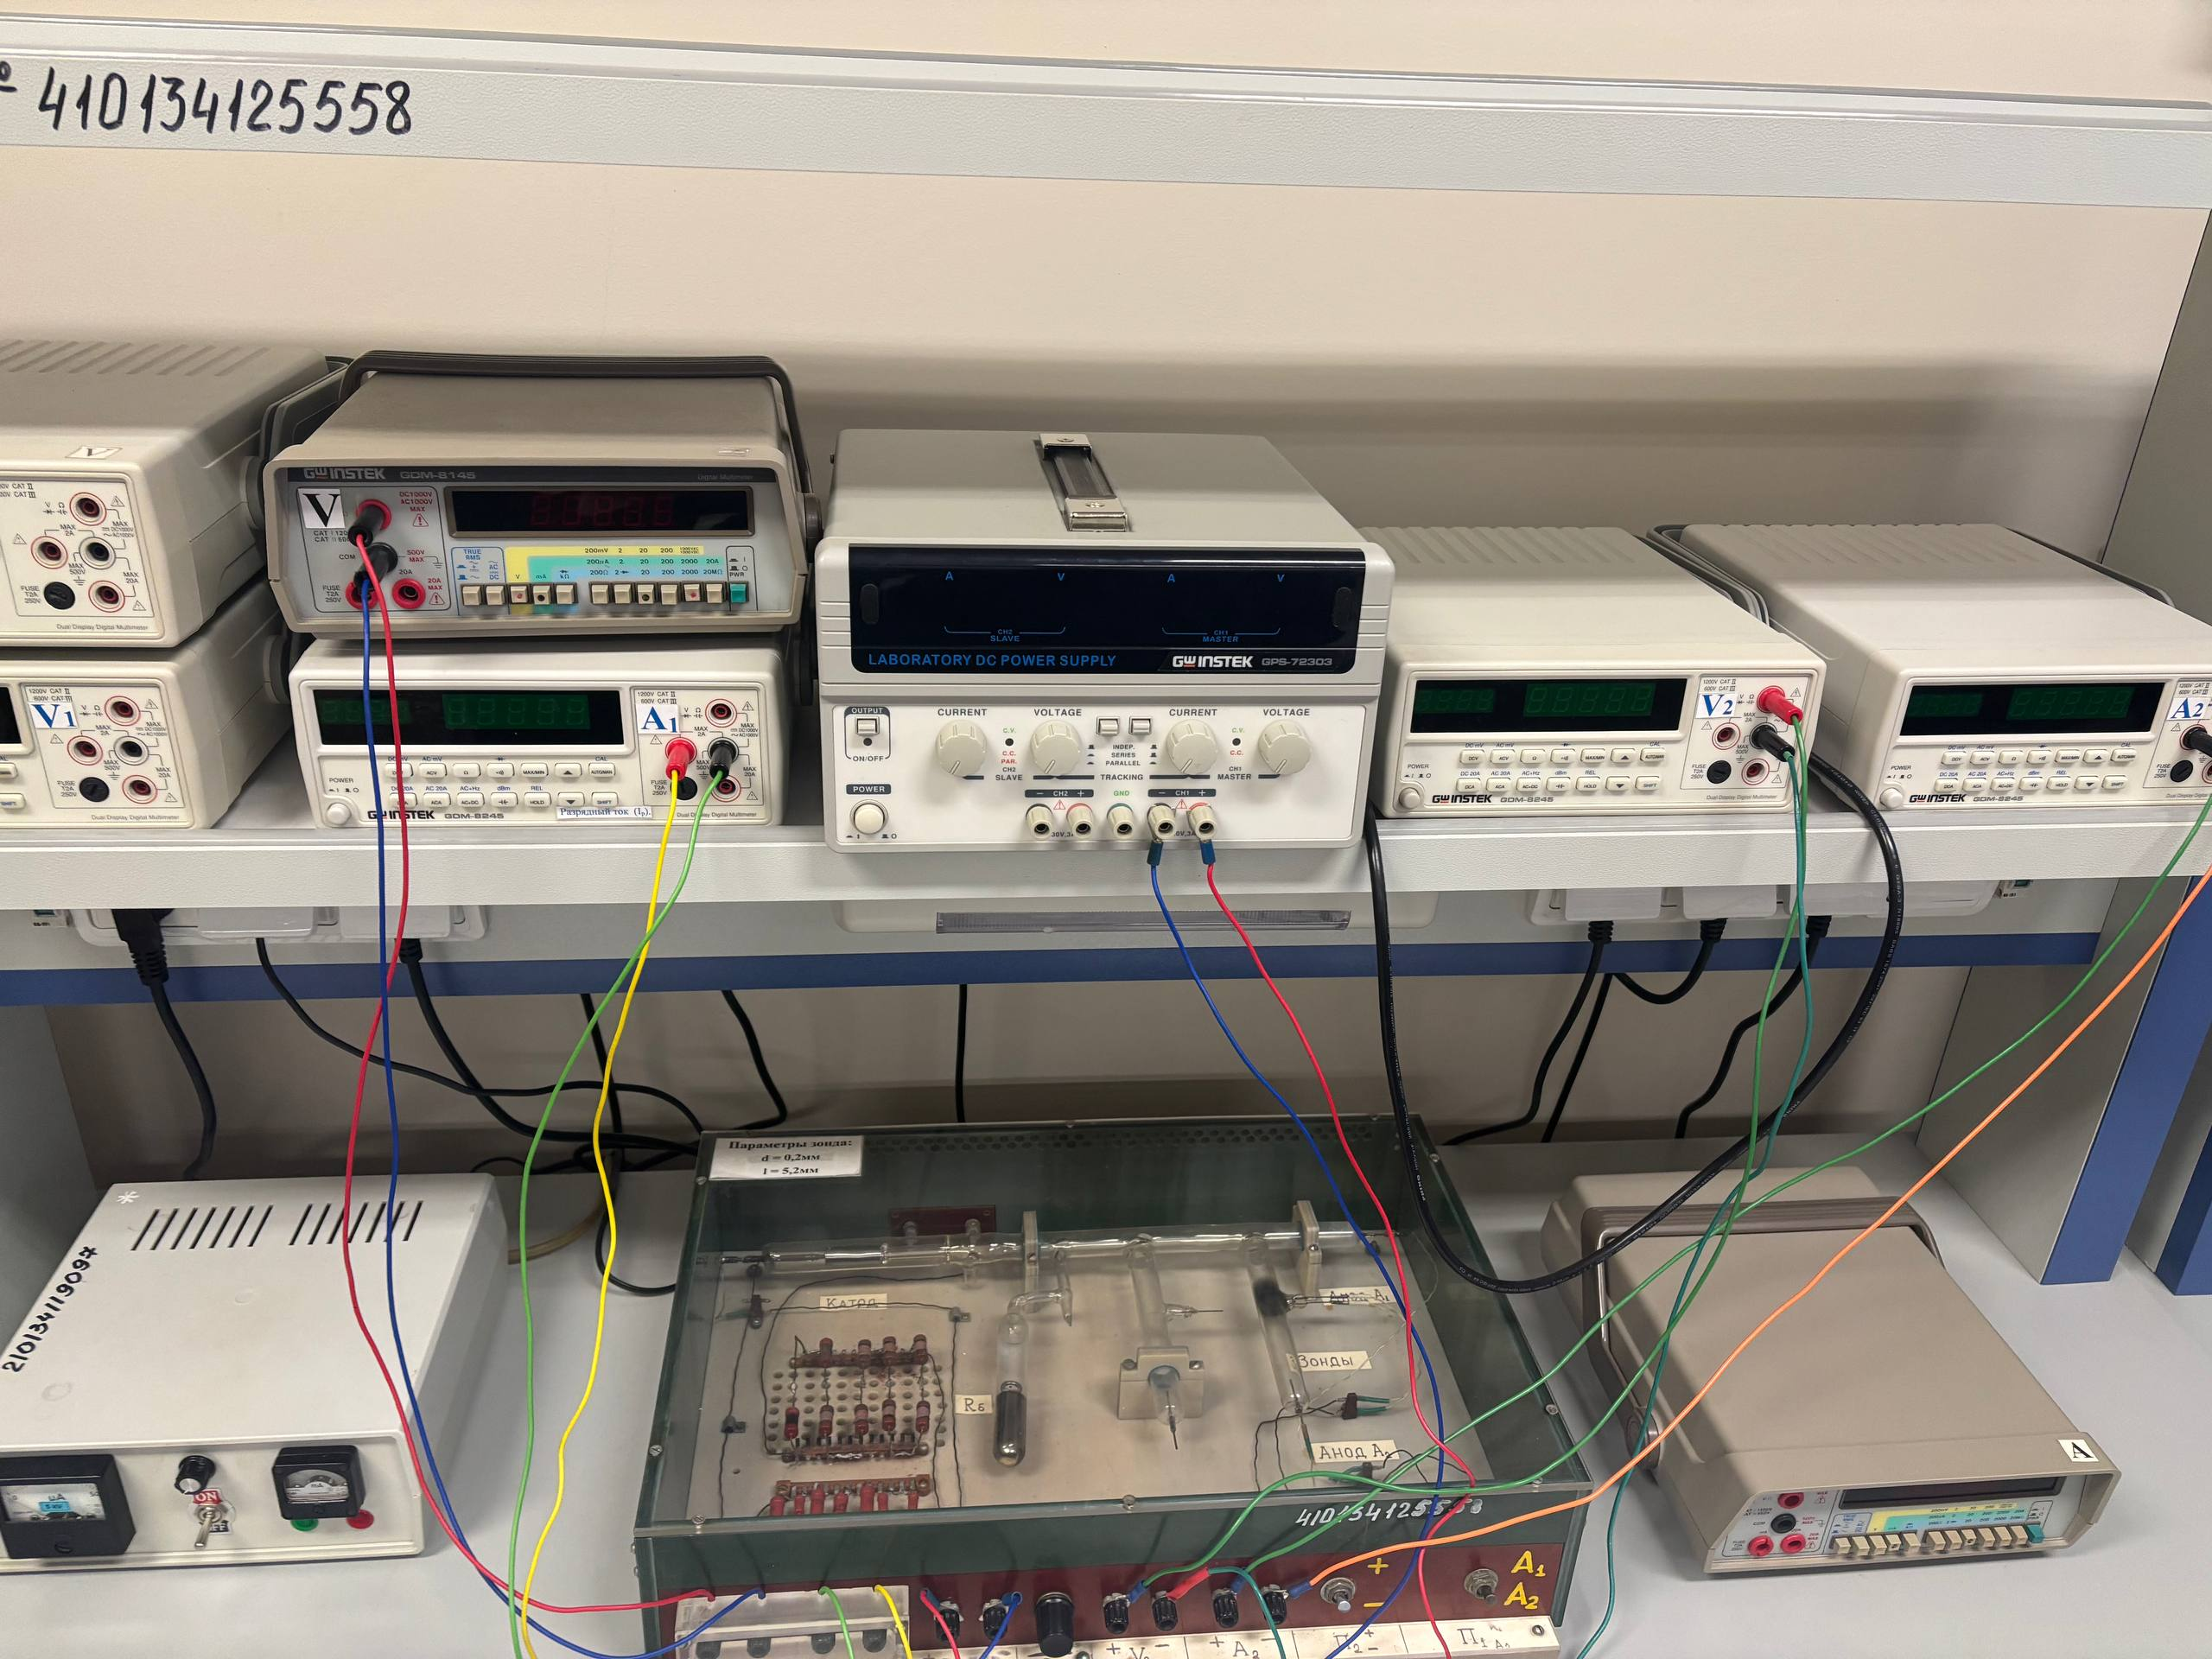
\includegraphics[width=.92\linewidth,height=.53\textheight,keepaspectratio]{img/setup.png}
\caption{Фотография установки, предоставленная автором. На табличке у трубки
указаны диаметр зонда 0,2 мм и длина 5,2 мм.}
\end{figure}
\clearpage
\subsection*{Принятая модель погрешностей}
По уточнению автора погрешность отсчёта равна одной единице последнего
записанного разряда $\delta x$, приборная составляющая равна $0{,}03|x|$.
Например, для $3{,}00$ мА принимается $\delta I=0{,}01$ мА,
для $1{,}5$ мА --- $\delta I=0{,}1$ мА. Пределы трактуются как полуширины
равномерных распределений, поэтому стандартная неопределённость показания
\[
 u(x)=\sqrt{\frac{\delta x^2+(0{,}03x)^2}{3}}.
\]
Это расчётное соглашение при отсутствии паспортных допусков.
Для каждого прибора $V_1,A_1,V_2,A_2$ принято одно общее смещение шкалы,
сохраняющееся между отсчётами, полярностями и режимами. Ошибки последнего
разряда считаются независимыми. В расчёте МНК распространены ошибки обеих
координат, включая корреляции отсчёта с вычисленным началом координат.

К приборной ковариации добавлена прежняя оценка разброса относительно
регрессии. Такое сложение консервативно, поскольку остатки могут частично
включать ошибки отсчётов. Таблицы и кресты на графиках показывают
стандартные неопределённости $u$, соответствующие одному среднеквадратическому
отклонению. Все номинальные точки и интервалы регрессии сохранены.
Параметры $d=0{,}2$ мм, $l=5{,}2$ мм, давление, температура ионов
и коэффициент делителя используются как заданные номиналы установки.
Допуски этих номиналов в бюджет не включены. Изменение метода учёта
сдвига полярностей рассмотрено отдельно в обсуждении.

Напряжение зажигания с учётом принятой модели равно
$U_{\text{заж}}=$ \input{\proc{ai_ignition.tex}} кВ.

\section{ВАХ разряда}
\else
\section{ВАХ разряда}
\fi
Для каждой ветви восстановлено $\Up=10U_{V_1}$. На \cref{fig:dis}
по горизонтали отложено напряжение на трубке. На большей части диапазона
точки прямого и обратного хода близки друг к другу.
\ifdefined\AIAppendix
Кресты на графике показывают стандартные неопределённости показаний
по принятой модели отсчёта и общей шкалы прибора.
\else
Классы точности приборов, пределы погрешности и допуск делителя в источниках
не приведены. На графиках отдельных отсчётов показаны исходные точки.
\fi
\begin{figure}[h!]\centering
\begin{tikzpicture}
\begin{axis}[lab,width=.76\linewidth,height=6.2cm,xlabel={$\Up$, В},
 ylabel={$\Ip$, мА},xmin=278,xmax=355,legend pos=north east]
\ifdefined\AIAppendix
\addplot[only marks,mark=o,labblue,mark size=2.2pt,probeerrors] table[col sep=comma,x=U_r_V,y=I_mA,x error=sU_r_V,y error=sI_mA]{\proc{ai_discharge_iv_up.csv}};
\else
\addplot[only marks,mark=o,labblue,mark size=2.2pt] table[col sep=comma,x=U_r_V,y=I_mA]{\proc{discharge_iv_up.csv}};
\fi
\addlegendentry{повышение тока}
\ifdefined\AIAppendix
\addplot[only marks,mark=+,labred,mark size=2.6pt,probeerrors] table[col sep=comma,x=U_r_V,y=I_mA,x error=sU_r_V,y error=sI_mA]{\proc{ai_discharge_iv_down.csv}};
\else
\addplot[only marks,mark=+,labred,mark size=2.6pt] table[col sep=comma,x=U_r_V,y=I_mA]{\proc{discharge_iv_down.csv}};
\fi
\addlegendentry{понижение тока}
\end{axis}
\end{tikzpicture}
\caption{Характеристика тлеющего разряда. Различные символы обозначают направление изменения тока.}\label{fig:dis}
\end{figure}

\clearpage
\subsection*{Дифференциальное сопротивление}
Для оценки $R_{\text{диф}}=d\Up/d\Ip$ данные каждой ветви упорядочены по току.
Прямая $\Up=a+R_{\text{диф}}\Ip$ проведена методом наименьших квадратов
(МНК) по каждому скользящему окну из трёх соседних точек.
В \cref{tab:r} сопоставлены наиболее крутой и наиболее пологий участки.
Один вольт на миллиампер соответствует одному килоому.
\begin{table}[h!]\centering
\caption{Экстремальные наклоны измеренной ВАХ. Интервалы тока заданы в мА, сопротивления в кОм.}
\label{tab:r}\small
\begin{tabular}{lcccc}
\hline
Ход & Интервал $\Ip$ & $R$ при $\max|R|$ & Интервал $\Ip$ & $\max R$\\ \hline
\inputrows{discharge_rows.tex}
\hline
\end{tabular}
\end{table}

Падение напряжения с ростом тока соответствует поднормальной части
тлеющего разряда (участок ГД на рис.~6 практикума~[3, с.~283--284]).
В нормальном режиме напряжение менялось бы мало. Балласт
стабилизирует рабочую точку при отрицательном дифференциальном сопротивлении.
Локальный наклон по трём отсчётам чувствителен к округлению напряжения и тока;
\ifdefined\AIAppendix
его неопределённость включает разброс относительно прямой при одной степени
свободы и распространение погрешностей обоих приборов. Окна экстремальных
наклонов выбраны по номинальным данным; неопределённость выбора окна не оценивалась.
\else
его статистическая ошибка характеризует разброс относительно прямой при одной степени свободы. Инструментальные ошибки в эту оценку не входят.
\fi

\section{Обработка зондовых характеристик}
Знак обеих координат восстановлен по положению П2. При почти нулевом
напряжении ветви оказываются смещены. Например, при $\Ip=4{,}99$~мА
получены $+11{,}4$~мкА при $+0{,}003$~В и $-9{,}2$~мкА при $-0{,}003$~В.
Секущая через эти два отсчёта дала бы $3{,}4\cdot10^3$~мкА/В,
тогда как на каждой ветви ток меняется всего на несколько мкА на вольт.
Поэтому при оценке наклона нужно отдельно учитывать сдвиг ветвей.
Для основной оценки использован графический метод п.~9 описания [1, с.~3]
с заменой построений линейным МНК. По точкам $U\ge16$~В и $U\le-16$~В
найдены две асимптоты $L_+(U)$ и $L_-(U)$, а по $|U|\le4{,}6$~В ---
общая центральная прямая $C(U)=gU+b$. Абсциссу центра $U_0$ определили
из условия $C(U_0)=[L_+(U_0)+L_-(U_0)]/2$.
На графиках $U'=U-U_0$, $I'=I-C(U_0)$,
а $\Is=[L_+(U_0)-L_-(U_0)]/2$.
Вычисленное по \eqref{eq:temp} значение соответствует половине расстояния
по горизонтали от оси $U'=0$ до пересечения касательной с уровнем $I'=\Is$.

Стандартные ошибки трёх прямых оценены по остаткам МНК. При переносе
в вычисляемые величины использована ковариация наклона и свободного члена
каждой прямой. Центральные и крайние точки принадлежат разным выборкам.
Влияние разрыва при смене полярности проверено повторной обработкой
с отдельным свободным членом для каждого положения П2.

\begin{table}[h!]\centering
\caption{Ионный ток насыщения, центральный наклон и энергия электронов.}\label{tab:probe}
\small\setlength{\tabcolsep}{5pt}
\begin{tabular}{ccccc}
\hline
$\Ip$, мА & $\Is$, мкА & $g$, мкА/В & $\kb T_e$, эВ & $\sigma_{T}/T_e$, \%\\ \hline
\inputrows{probe_rows.tex}
\hline
\end{tabular}
\end{table}

\clearpage
\subsection*{Измеренные точки и построения}
\begin{figure}[h!]\centering
\resizebox{.47\linewidth}{!}{\probepanel{3}{1{,}50}}\hfill\resizebox{.47\linewidth}{!}{\probepanel{2}{3{,}00}}
\par\medskip
\probepanel{1}{4{,}99}
\caption{Характеристики двойного зонда в центрированных координатах.
Штриховые прямые показывают экстраполяцию крайних ветвей, сплошные --- наклон вблизи нуля.}
\label{fig:individual}
\end{figure}
\begin{figure}[h!]\centering
\begin{tikzpicture}
\begin{axis}[lab,width=.80\linewidth,height=6.5cm,xlabel={$U'$, В},
 ylabel={$I'$, мкА},legend pos=north west,legend style={font=\footnotesize}]
\ifdefined\AIAppendix
\addplot[only marks,mark=triangle*,labgreen,mark size=1.6pt,probeerrors] table[col sep=comma,x=U_c_V,y=I_c_uA,x error=sU_c_V,y error=sI_c_uA]{\proc{ai_probe_centered_3.csv}};
\else
\addplot[only marks,mark=triangle*,labgreen,mark size=1.6pt] table[col sep=comma,x=U_c_V,y=I_c_uA]{\proc{probe_centered_3.csv}};
\fi
\addlegendentry{$1{,}50$ мА}
\ifdefined\AIAppendix
\addplot[only marks,mark=square*,labred,mark size=1.35pt,probeerrors] table[col sep=comma,x=U_c_V,y=I_c_uA,x error=sU_c_V,y error=sI_c_uA]{\proc{ai_probe_centered_2.csv}};
\else
\addplot[only marks,mark=square*,labred,mark size=1.35pt] table[col sep=comma,x=U_c_V,y=I_c_uA]{\proc{probe_centered_2.csv}};
\fi
\addlegendentry{$3{,}00$ мА}
\ifdefined\AIAppendix
\addplot[only marks,mark=*,labblue,mark size=1.5pt,probeerrors] table[col sep=comma,x=U_c_V,y=I_c_uA,x error=sU_c_V,y error=sI_c_uA]{\proc{ai_probe_centered_1.csv}};
\else
\addplot[only marks,mark=*,labblue,mark size=1.5pt] table[col sep=comma,x=U_c_V,y=I_c_uA]{\proc{probe_centered_1.csv}};
\fi
\addlegendentry{$4{,}99$ мА}
\end{axis}\end{tikzpicture}
\caption{Семейство зондовых характеристик в одной системе координат.}\label{fig:family}
\end{figure}

\clearpage
\section{Параметры плазмы и обсуждение}
Для перевода энергии в температуру использовано $1~\text{эВ}/\kb\simeq
11\,605$~К. Электронную концентрацию рассчитали по \eqref{eq:bohm},
параметры экранирования --- по \eqref{eq:lengths}.
Погрешности в таблицах относятся к обработке зондовых характеристик
при фиксированных номиналах $d,l,P,T_i$. Вариации показаний при смене
полярности и неопределённость выбора диапазона МНК влияют на точность
центрального наклона.

\begin{table}[h!]\centering
\caption{Температура, концентрация и частоты электронных колебаний.}\label{tab:base}
\small\setlength{\tabcolsep}{4.5pt}
\begin{tabular}{ccccc}\hline
$\Ip$, мА & $T_e$, $10^3$ К & $n_e$, $10^{10}$ см$^{-3}$ & $\omega_p$, $10^9$ рад/с & $f_p$, МГц\\ \hline
\inputrows{plasma_base_rows.tex}
\hline\end{tabular}
\end{table}
\begin{table}[h!]\centering
\caption{Характеристики экранирования и степень ионизации.}\label{tab:debye}
\small
\begin{tabular}{ccccc}\hline
$\Ip$, мА & $r_{De}$, мкм & $r_D$, мкм & $N_D$ & $\alpha$, $10^{-7}$\\ \hline
\inputrows{plasma_debye_rows.tex}
\hline\end{tabular}
\end{table}

\begin{figure}[h!]\centering
\begin{tikzpicture}
\begin{axis}[lab,width=.485\linewidth,height=5.5cm,xlabel={$\Ip$, мА},ylabel={$\kb T_e$, эВ},xmin=1,xmax=5.5]
\ifdefined\AIAppendix
\addplot[only marks,mark=*,labblue,error bars/.cd,y dir=both,y explicit,x dir=both,x explicit]
 table[col sep=comma,x=Ip_mA,y=Te_eV,y error=sTe_eV,x error=sIp_mA]{\proc{ai_plasma_params.csv}};
\else
\addplot[only marks,mark=*,labblue,error bars/.cd,y dir=both,y explicit]
 table[col sep=comma,x=Ip_mA,y=Te_eV,y error=sTe_eV]{\proc{plasma_params.csv}};
\fi
\end{axis}
\end{tikzpicture}\hfill
\begin{tikzpicture}
\begin{axis}[lab,width=.485\linewidth,height=5.5cm,xlabel={$\Ip$, мА},ylabel={$n_e$, $10^{10}$ см$^{-3}$},xmin=1,xmax=5.5]
\ifdefined\AIAppendix
\addplot[only marks,mark=square*,labred,error bars/.cd,y dir=both,y explicit,x dir=both,x explicit]
 table[col sep=comma,x=Ip_mA,y=n_1e10_cm3,y error=sn_1e10_cm3,x error=sIp_mA]{\proc{ai_plasma_params.csv}};
\else
\addplot[only marks,mark=square*,labred,error bars/.cd,y dir=both,y explicit]
 table[col sep=comma,x=Ip_mA,y=n_1e10_cm3,y error=sn_1e10_cm3]{\proc{plasma_params.csv}};
\fi
\end{axis}
\end{tikzpicture}
\caption{Электронная температура в энергетических единицах и концентрация.
\ifdefined\AIAppendix
Кресты показывают стандартные неопределённости тока разряда и рассчитанных параметров.
\else
Вертикальные отрезки показывают расчётную неопределённость.
\fi}\label{fig:trend}
\end{figure}
\clearpage
\subsection*{Пределы точности и физическая интерпретация}
Измеренный ток насыщения растёт от $16{,}73$ до $67{,}2$~мкА.
При сравнимых энергиях электронов это соответствует росту концентрации
почти в четыре раза (\cref{tab:base}). Рост числа носителей заряда
согласуется с увеличением тока разряда. По трём режимам отдельный закон
зависимости концентрации от тока установить трудно.

Для проверки устойчивости обработки полуширину центрального участка
поочерёдно заменяли на $3$ и $6{,}5$~В, границу крайних участков ---
на $15$ и $18$~В. Менялся один параметр за один расчёт. При токах
$1{,}50$, $3{,}00$ и $4{,}99$~мА энергии при таком выборе составили
$3{,}25$--$3{,}57$, $3{,}33$--$3{,}96$ и $2{,}54$--$3{,}86$~эВ
\ifdefined\AIAppendix
соответственно. До подтверждения рукописи автором дополнительно исключали
десять первоначально спорных отсчётов, что меняло оценки на
$0{,}06$--$0{,}09$~эВ. Автор подтвердил все принятые значения;
в итоговый расчёт входят все 83 точки.
\else
соответственно. Исключение отсчётов с неоднозначно прочитанными цифрами
изменило основные оценки примерно на $0{,}06$--$0{,}09$~эВ.
\fi

Если при тех же крайних участках и фиксированном $\Is$ аппроксимировать
центральные точки прямыми с общим наклоном и двумя разными свободными
членами, получаются $3{,}50$, $4{,}31$ и $5{,}20$~эВ. При максимальном
токе поправка достигает $49\,\%$, существенно превышая стандартную ошибку
основного построения. Журнал не позволяет установить причину сдвига ветвей.
Поэтому зависимость температуры от тока по этим данным неоднозначна.

Для всех режимов $T_e$ существенно выше $T_i$.
Электронная поляризационная длина равна $0{,}058$--$0{,}112$~мм.
Даже длина зонда $5{,}2$~мм превышает её примерно в 46--90 раз, что
согласуется с квазинейтральностью объёма положительного столба на
миллиметровых масштабах. Радиус самой трубки в журнале не указан.
В сфере экранирования находится около 30--59 ионов; по принятому в
описании критерию $N_D\gg1$ запас составляет несколько десятков. Это позволяет использовать приближение идеальной плазмы.
Доля ионизованных атомов остаётся меньше $10^{-6}$ во всех трёх режимах.

\section{Заключение}
В диапазоне $0{,}51$--$5{,}01$~мА получена падающая ВАХ разряда.
\ifdefined\AIAppendix
Наибольший по модулю локальный наклон приведён с расширенным бюджетом неопределённости в \cref{tab:r}
\else
Наибольший по модулю локальный наклон равен $(-31{,}4\pm3{,}3)$~кОм
\fi
при понижении тока, на интервале $0{,}51$--$0{,}77$~мА.
Зондовая диагностика дала концентрацию от $1{,}48\cdot10^{10}$ до
$5{,}80\cdot10^{10}$~см$^{-3}$.
При этом частота отсечки возросла с $1{,}09$ до $2{,}16$~ГГц.
Основная оценка энергии электронов составляет $3{,}3$--$3{,}7$~эВ;
наиболее существенное ограничение её точности связано со смещением
зондового тока при переключении полярности.

\section*{Источники}
\begin{enumerate}
\item \textit{3.5.1 (4.16). Изучение плазмы газового разряда в неоне.
Дополнительное описание}. Редакция от 11 августа 2021~г.
С.~1 (установка), с.~2--3 (измерения), с.~3--4 (обработка).
\item Лабораторный журнал работы 3.5.1 (4.16), 17.11.2026.
С.~1 --- ВАХ разряда и первая полярность серии $4{,}99$~мА;
с.~2--3 --- продолжение зондовых измерений. Первичные числовые данные
доступны по адресу \url{https://github.com/duxihw/labs_lpr/tree/main/3.5.1/data/raw}.
\item Никулин М.~Г., Попов П.~В., Нозик А.~А. и др.
\textit{Лабораторный практикум по общей физике. Т.~2. Электричество и магнетизм}.
Под ред. А.~В.~Максимычева и М.~Г.~Никулина. 2-е изд.
М.~: МФТИ, 2019. С.~283--284, рис.~6. ISBN 978-5-7417-0709-8.
\end{enumerate}


\ifdefined\AIAppendix\AIAppendix\fi
\end{document}
